In this section, we show empirical results of our algorithm on different transferring situations on two datasets: AwA\footnote{The features of AwA dataset is available from http://attributes.kyb.tuebingen.mpg.de/} \cite{lampert2009learning} and Caltech-256\footnote{Images for Caltech-256 is available from http://www.vision.caltech.edu/Image\_Datasets/Caltech256/} \cite{griffin2007caltech}. We design the following \hl{3 sets of experiments: learning from informative prior (positive transfer), unrelated prior (negative transfer) and mixed prior (negative transfer), } to show the effectiveness of our algorithm.
\subsection{Dataset}
Caltch-256 contains 30607 images from 256 categories. We select the following 10 categories: \textit{bat, bear, dolphin, giraffe, gorilla, horse, leopard, raccoon, skunk, zebra}, containing 1387 images, as our dataset.

AwA dataset consists of 50 animal categories. Its source images is not publicly accessible and we can only access the six pre-extracted feature representations for each image. This property makes it natural as the unknown distribution source dataset to train the prior knowledge. We choose the identical 10 categories as those in Caltech-256 from it, containing 6917 images.

\subsection{Baselines and algorithmic setup}
We compare our algorithm with two kinds of baselines. The first one is methods without leveraging any prior knowledge (no transfer baselines). The second consists of some methods with transfer techniques. Here are the no transfer baselines.

\textbf{No transfer:} LS-SVM trained only on target data. This baseline can be the indicator as the best performance in the \hl{bad oracle experiment.}

\textbf{Batch:} \hl{This baseline is only used in good oracle experiment.} We combined the source and target data, assuming that we have fully access to all data, to train the LS-SVM. The result of this baseline might be considered as the best performance achieved in the experiment as well as an important reference for assessing the models with transfer learning methods.

\textbf{Source+1:} This method only train a new binary LS-SVM for the new category. For the rest of the classes, we use the predictions of the classifiers trained from source data directly. This is arguably the easiest way for transfer learning. \hl{In some of our experiments, it is a good indicator when negative transfer happens.}

We select the following 3 methods as our transfer baselines. The general property of these 3 methods is that they all try to leverage multiple prior knowledge to benefit the transfer procedure.

\textbf{MKTL \cite{jie2011multiclass}:} This method uses the output of prior models as extra feature inputs, and automatically determine from which prior models to transfer and how much to transfer.


\textbf{MULTI-KT \cite{tommasi2014learning}:} This method has similar idea with MKTL. It uses LOO error to determine how much to transfer from prior models and convert it into solving the convex optimization problem.

\textbf{MULTIpLE \cite{kuzborskij2013n}:} The basic setting of this method is similar like ours. It is designed to balance the performance between learning the new category and preserving the model from prior knowledge.

For all the experiments in this section, we used kernel averaging \cite{gehler2009feature}, computing the average of RBF kernels over the available features on RBF hyperparameter $\{2^{-5},2^{-4},...,2^8\}$. The penalty parameter $C$ is tuned via cross-validation on $\{10^{-5},10^{-4},...,10^8\}$ and the optimal value is reused for all the algorithms.

\subsection{Transfer the knowledge from highly related knowledge}

In MITL, the categories in both source and target task are drawn from the same distribution. Despite the affect of the new added category, transferring knowledge from prior knowledge can be considered as positive transfer. We perform the experiment under this scenario on both AwA and Caltech. On each dataset, we iteratively choose one category as the new category and run multiple times to get the average performance of each algorithm. The results of these two datasets are reported in Table \ref{tab:C2C} and Table \ref{tab:A2A}. From the result we can see that, in Caltech experiment, our algorithm consistently outperforms all the baselines even better than Batch.

To illustrate the detail performance of our algorithm, we select the experiment result on AwA dataset where horse is chosen as the new category for further explanation. In Figure \ref{fig:awa-a}, we show the average performances of different methods on different training size for 10 experiments. We can observe that, as the training size increases, our method can even outperforms the batch method.
In Figure \ref{fig:awa-b} we provide values of $\gamma$ and $\beta$ compared with the parameters of the runner-up transfer algorithm MULTIpLE. We can see that for transfer knowledge between identical categories, MULTIpLE fixes the transfer parameter ($\gamma$) to be 1 while our method sets greater weights for related prior knowledge. The same phenomenon is observed for the transfer parameter $\beta$. By exploiting the positive prior knowledge more aggressively, SMITLe is able to leverage the prior knowledge and outperforms other methods. In Table \ref{tab:A2A}, \hl{Source+1 outperforms SMITLe when the training size is small. This could be due to the noisy examples. As we increase the training size, the accuracy of SMITLe increases and outperforms Source+1. }


\begin{figure*}
\centering
\subfloat[Overall accuracy comparision with different baselines. ]{\includegraphics[scale=.4]{fig/A2A_horse.eps}\label{fig:awa-a}}
\subfloat[Comparision with MULTIpLE.] {\includegraphics[scale=0.4]{fig/A2A_gama.eps}\label{fig:awa-b}}

\caption{Experiment results for 10 classes, AwA. Horse is used as the new category. \protect\subref{fig:awa-a}}
\label{fig:awa}
\end{figure*}


\begin{table}[htbp]
  \centering
  \caption{Average performance from Caltech to Caltech with different size of training set in target problem. 30 examples are randomly chosen from each class to train the source classifier and 30 examples from each class are chosen for test. }
    \begin{tabular}{ccccc}
    \toprule
      size per category    & 5     & 10    & 15    & 20 \\
    \midrule
    No transfer &         27.33  &         31.53  &         35.73  &         38.47  \\
    Source+1    &         43.33  &         43.87   &         44.33  &         44.57   \\
    MKTL        &         38.89  &         43.27   &         45.72  &         47.44   \\
    MULTIKT     &         37.96  &         42.89   &         45.96  &         47.32  \\
    MULTIpLE    &         42.63  &         45.63   &         47.81  &         48.73 \\
    SMITLe        &         \textbf{43.53 }&         \textbf{46.45 } &         \textbf{48.25 } &         \textbf{49.15 } \\
        \midrule
    Batch       &         43.77  &         44.73   &         46.67  &         48.00 \\
    \bottomrule
    \end{tabular}%
  \label{tab:C2C}%
\end{table}%

% Table generated by Excel2LaTeX from sheet 'Sheet1'
\begin{table}[htbp]
  \centering
  \caption{Average performance from AwA to AwA with different size of training set in target problem. 50 examples are randomly chosen from each class to train the source classifier and 200 examples from each class are chosen for test.}
    \begin{tabular}{ccccc}
    \toprule
     size per category    & 5     & 10    & 15    & 20 \\
    \midrule
    No transfer &         23.52  &         26.79  &         29.60  &         31.50  \\
    Source+1    &         \textbf{39.00 } &         \textbf{39.34 } &         39.62 &         39.74  \\
    MKTL        &         31.46  &         34.76  &         37.41  &         38.81  \\
    MULTIKT     &         29.86  &         32.86  &         35.22  &         36.33  \\
    MULTIpLE    &         37.80  &         38.81  &         39.80  &         40.47  \\
    SMITLe        &        {37.83 } &         {39.31 } &         \textbf{40.37 } &         \textbf{41.09} \\
        \midrule
    Batch       &         39.62  &         40.18  &         40.67  &         41.44  \\
    \bottomrule
    \end{tabular}%
  \label{tab:A2A}%
\end{table}%



\subsection{Transfer the knowledge from unrelated knowledge}
In this section, we show how our method performs in transferring knowledge between two different datasets, from AwA to Caltech. Following the settings in previous section, the prior models are trained from AwA dataset and we iteratively select one category as the new one, running multiple times to get the average results for all the algorithms. We show the average performance of each algorithm in Table \ref{tab:A2C}. 

Still we take the experiment where horse is considered as the new category to see the detail performance of each algorithm. In Figure \ref{fig:a2c-a} we can see that, the accuracy of Source+1 is much lower than no transfer, which indicates that the knowledge from prior AwA is unrelated to Caltech dataset. From here we can see that, not surprisingly, the accuracy of SMITLe shows similar accuracy to the no transfer baseline, while other methods suffer from negative transfer and perform even worse than no transfer baseline.  In Figure \ref{fig:awa-b} we show the parameters learned for each classes in SMITLe in comparison with MULTIpLE. We can see that, when the prior knowledge is unrelated, SMITLe resists utilizing the prior knowledge and therefore shows almost identical accuracy to the no transfer baseline.
%\begin{figure*}
%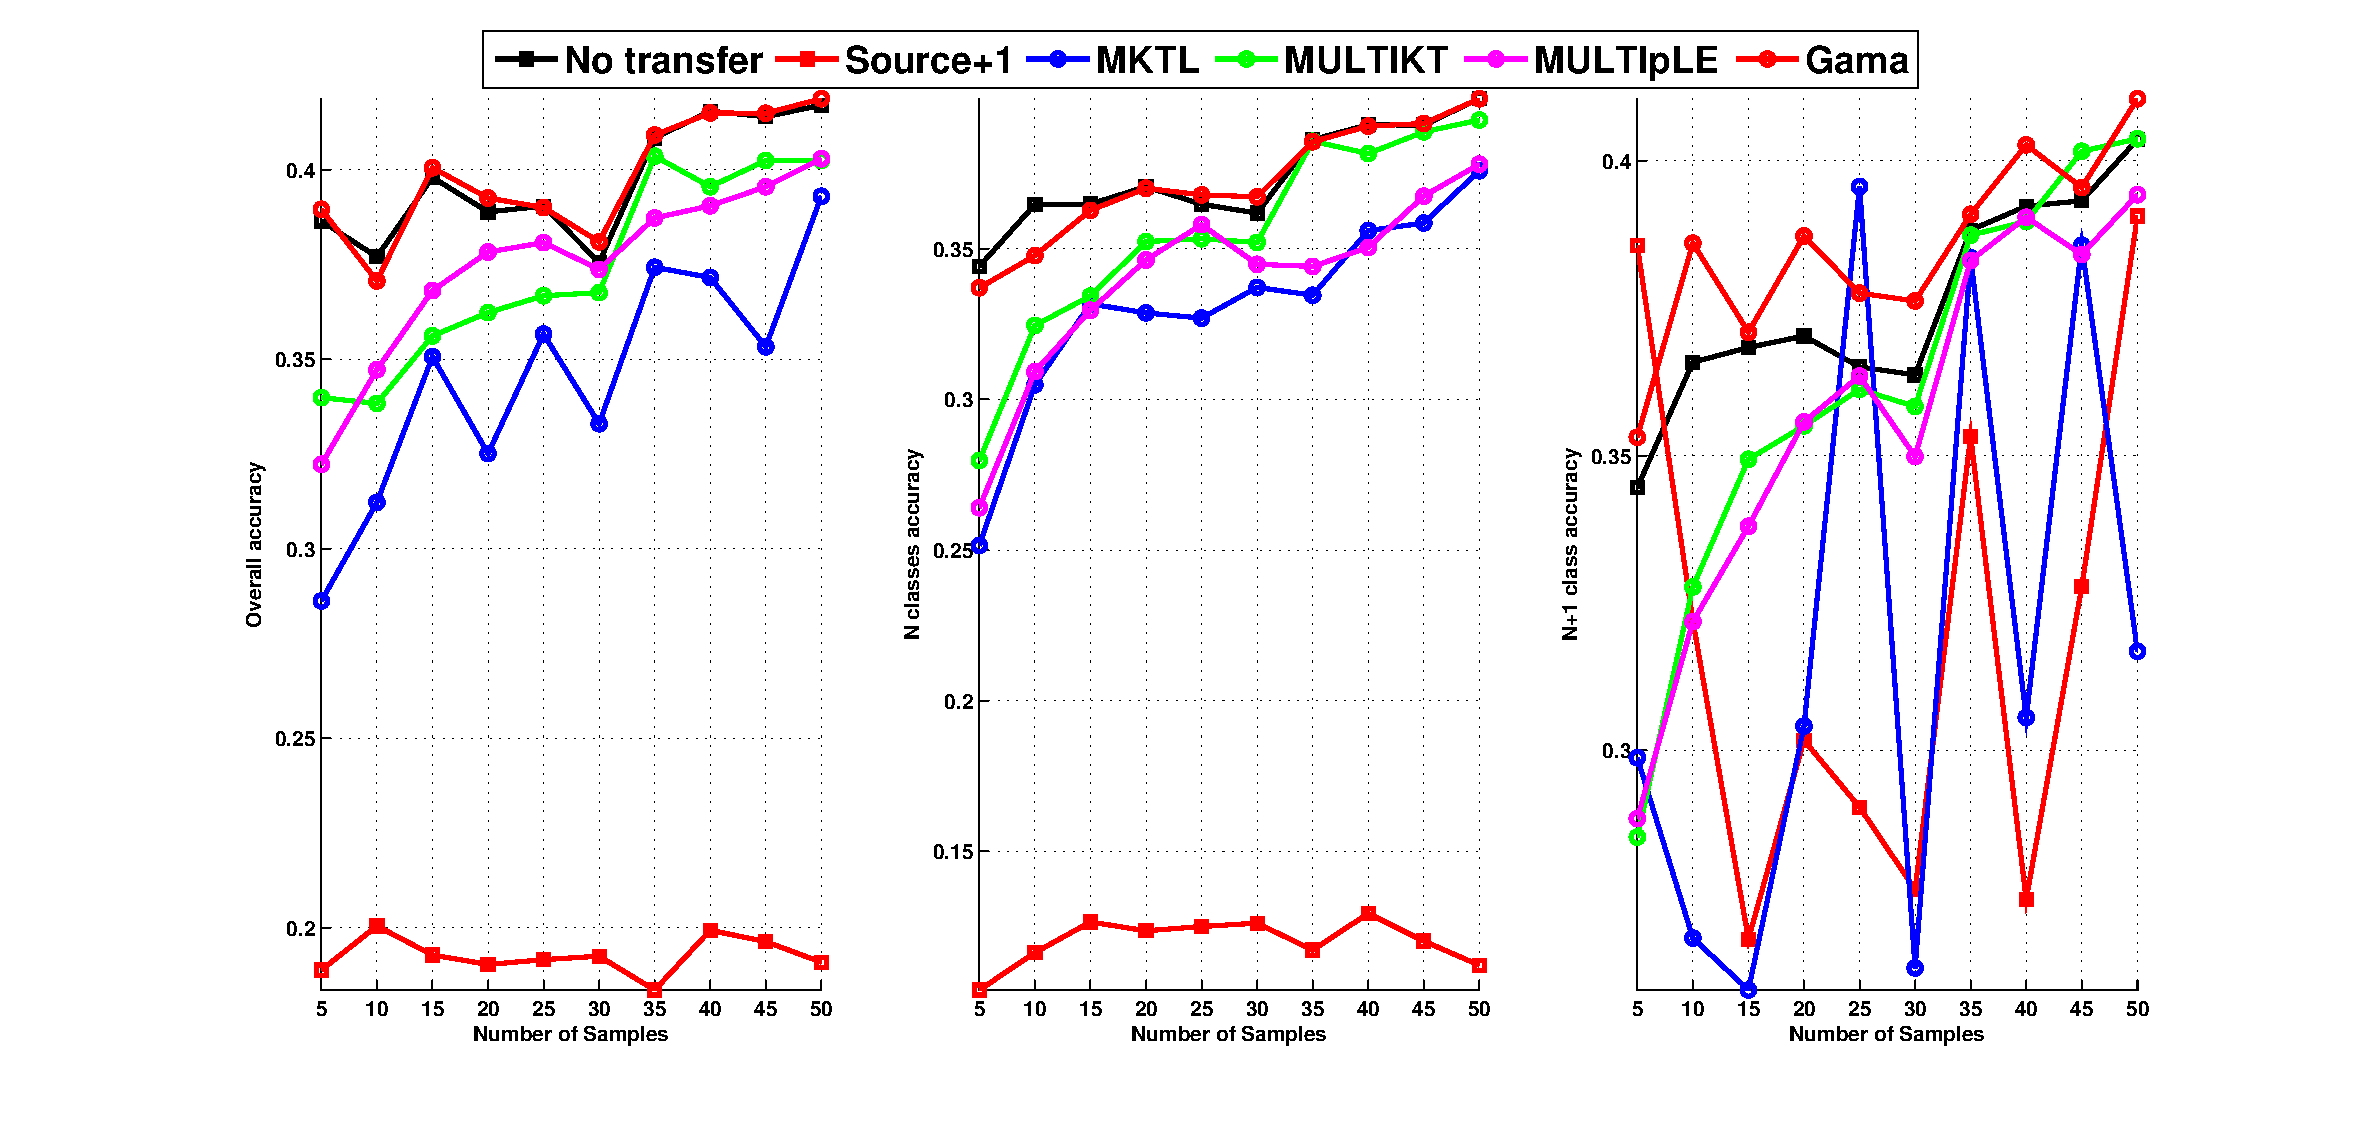
\includegraphics[width=\textwidth,height=5cm]{fig/A2C_RBF_PHOG.eps}
%\caption{Transferring from AwA to Caltech-256.}
%\end{figure*}
% Table generated by Excel2LaTeX from sheet 'Sheet1'

\begin{figure*}
	\centering
	\subfloat[Overall accuracy comparision with different baselines. ]{\includegraphics[scale=.4]{fig/A2C_horse.eps}\label{fig:a2c-a}}
	\subfloat[Comparision with MULTIpLE.] {\includegraphics[scale=0.4]{fig/A2C_gama.eps}\label{fig:a2c-b}}
	\caption{Experiment results for 10 classes, AwA. Horse is used as the new category. \protect\subref{fig:a2c-a}}
	\label{fig:a2c}
\end{figure*}


\begin{table}[htbp]
  \centering
  \caption{Average performance from AwA to Caltech. Examples in AwA are used to train prior models. Different number of training size is randomly selected from Caltech dataset.}
    \begin{tabular}{ccccccc}
    \toprule
                & 5              & 10             & 15             & 20             & 25             & 30 \\
    \midrule
    No transfer &         \textbf{30.99 } &         33.97  &         35.95 &         37.78  &         38.27  &         39.39  \\
    Source+1    &         17.89  &         18.69  &         18.79  &         19.69  &         19.39  &         20.20  \\
    MKTL        &         25.19  &         30.14  &         32.53  &         34.30  &         35.83  &         36.66  \\
    MULTIKT     &         27.60  &         32.19  &         34.51  &         36.78  &         37.79  &         39.27  \\
    MULTIpLE    &         29.79  &         33.45  &         35.49  &         36.77  &         37.43  &         38.62  \\
    SMITLe        &       30.93  &         \textbf{34.13 } &         \textbf{36.09 } &         \textbf{38.01} &         \textbf{38.46} &         \textbf{39.59} \\
    \bottomrule
    \end{tabular}%
  \label{tab:A2C}%
\end{table}%

\subsection{mixed}

\begin{figure*}
  \centering
  \subfloat[]{    \includegraphics[width=0.18\textwidth]{fig/A2A_bad/A2A_bad3.eps}  }
  \subfloat[]{    \includegraphics[width=0.18\textwidth]{fig/A2A_bad/A2A_bad2.eps}  }
  \subfloat[]{    \includegraphics[width=0.18\textwidth]{fig/A2A_bad/A2A_bad1.eps}  }
  \subfloat[]{    \includegraphics[width=0.18\textwidth]{fig/A2A_bad/A2A_bad4.eps}  }
  \subfloat[]{    \includegraphics[width=0.18\textwidth]{fig/A2A_bad/A2A_bad5.eps}  }\\
  \subfloat[]{    \includegraphics[width=0.18\textwidth]{fig/A2A_bad/A2A_bad6.eps}  }
  \subfloat[]{    \includegraphics[width=0.18\textwidth]{fig/A2A_bad/A2A_bad7.eps}  }
  \subfloat[]{    \includegraphics[width=0.18\textwidth]{fig/A2A_bad/A2A_bad8.eps}  }
  \subfloat[]{    \includegraphics[width=0.18\textwidth]{fig/A2A_bad/A2A_bad9.eps}  }
  \subfloat[]{    \includegraphics[width=0.18\textwidth]{fig/A2A_bad/A2A_bad10.eps}  }\\
  \caption{A2A bad, 4 classes }
\end{figure*}

\begin{figure*}
  \centering
  \subfloat[]{    \includegraphics[width=0.18\textwidth]{fig/A2A_bad/A2A_bad_3c_3.eps}  }
  \subfloat[]{    \includegraphics[width=0.18\textwidth]{fig/A2A_bad/A2A_bad_3c_2.eps}  }
  \subfloat[]{    \includegraphics[width=0.18\textwidth]{fig/A2A_bad/A2A_bad_3c_1.eps}  }
  \subfloat[]{    \includegraphics[width=0.18\textwidth]{fig/A2A_bad/A2A_bad_3c_4.eps}  }
  \subfloat[]{    \includegraphics[width=0.18\textwidth]{fig/A2A_bad/A2A_bad_3c_5.eps}  }\\
  \subfloat[]{    \includegraphics[width=0.18\textwidth]{fig/A2A_bad/A2A_bad_3c_6.eps}  }
  \subfloat[]{    \includegraphics[width=0.18\textwidth]{fig/A2A_bad/A2A_bad_3c_7.eps}  }
  \subfloat[]{    \includegraphics[width=0.18\textwidth]{fig/A2A_bad/A2A_bad_3c_8.eps}  }
  \subfloat[]{    \includegraphics[width=0.18\textwidth]{fig/A2A_bad/A2A_bad_3c_9.eps}  }
  \subfloat[]{    \includegraphics[width=0.18\textwidth]{fig/A2A_bad/A2A_bad_3c_10.eps}  }\\
  \caption{A2A bad, 3 classes }
\end{figure*}
